\section{Methodology}
%Redo research methodology section.
%Redo data analysis section.

\subsection{Research methodology}
%Research methodology description

% 1.2 Provide a problem statement with a strong hypothesis / Define your methodological approach 
 In order to ensure the validity of the findings from experimentation in the virtual network lab and also create a testing framework which can be used to benchmark contemporary network scanning methods in the future, a multi-factorial approach will be employed. This includes a purposeful sample selection; topologies most commonly found in real world networks will be implemented, consisting of structures sourced from the Internet Topology Zoo\cite{topology_zoo}. Furthermore, a robust enumeration of macros across all possible network shapes will be explored, this will likely increase the available search space covered by the evaluation, through testing and evaluating the edge cases. Using this approach has the benefit of possibly highlighting potential flaws and unexpected behaviour of current methods, in a way that using conventional structures might not. To achieve stochastic network generation, the Erdos-Renyi and Barabasi-Albert models have been employed. By combining both  'real-world' and theoretical network topology structures, the proposed network lab has the advantages of improved versatility and coverage of yielded data.  

Contemporary tools used to map network topologies such as Paristraceroute\cite{anomalies} and DiamondMiner\cite{diamond-miner} have improved on the original traceroute. However, these contemporary methods still have deficiencies, suggesting that there is still potential for these tools to be extended to mitigate these flaws. Thorough analysis of results from the literature and also from experimentation in an optimally configured virtually implemented lab, can potentially form the basis of the proposed improvements to the contemporary methods. This highlights the importance of having the network lab parameters optimally configured, to allow effective evaluation. Furthermore, an effective testing environment is not limited to measuring the performance of network scanning tools, and has other applications ranging from testing different protocols and router images. 

% 3. State research design
\subsection{Research methods}
%Research methods description
Evaluation of the varying topology structures will be primarily quantitative. With comparison between each equivalently sized topology structures being carried out using the shortest path difference and degree correlation. This evaluation will seek to establish if randomly generated topologies can capture the characteristics of real-world networks, and if so what is the optimal configuration. 

The proposed virtual lab environment will be implemented primarily using ContainerLab \cite{containerlab} which is an open source network emulator which allows the creation of virtual network environments, leveraging the powerful docker framework, it supports containerized router images of products offers by major companies such as Cicso, Juniper and Dell. Alpine Linux for the purpose of this research project, will be used as an example for the container images, due to it's low running constraints compared with similar Linux distributions such as Debian\cite{alpine} and open-source code base. This mitigates any potential memory concerns when simulating more complex network topologies. Furthermore, by evaluating contemporary tools or otherwise in a virtual network lab the experiment variables are fully controllable, allowing for repeatable results and avoidance of external interference. By using a virtual environment the possibility of numerous results being collected for each configuration are ensured, allowing statistical analysis of the results to be carried out. This further increases the validity of the evaluation. Additionally, by simulating the network topologies ethical implications of evaluating performance on the real-world internet are avoided. 

% 4. Discuss specifics of data collection and methodology

% 5. Justify methods used - mention limitations, strengths and weaknesses.

\subsection{Virtual Network lab}
To facilitate evaluation of contemporary network scanning tools, using the a virtual network lab has been created. The implemented virtual network lab was created inside a virtual machine running the Debian based Linux Operating System  Kali Linux. 

Using this approach allows for an isolated testing environment, avoiding external factors which could interfere with the experimental results. Furthermore, by employing a virtual lab complete control and configuration of the experimental variables is ensured. Due to this the experimental results can be replicated a number of times, increasing the validity of the findings. 

Additionally, due to the portability of virtual machines across varying Operating systems, the configuration and findings from this research can be readily built upon and revised, encouraging more work in this area.

In order to measure and compare the performance of tools utilised to map network topologies in an objective manner, a standardised testing environment should be employed. Creation and design of this given testing environment will be based upon a multi-factorial approach; by utilising structures which are representative of real world network topology, using configurations such as so-called "star" and "bus" topologies will ensure a realistic measurement of expected performance with a high probability of confidence due to their prevalence across many varying topologies. 

Additionally, in conjunction with the practical real-world approach, a robust enumeration of all possible network shapes will be employed to increase the available performance search space of each tool in topology measurement. Utilising this stochastic approach allows for potential edge cases to be identified, possibly highlighting previously unknown design flaws/weaknesses in a given tool. 

\subsection{Topology models}
Below, a description and evaluation for each of the basic network topology model types will be given. This is to give the reader further context about the structural and behavioural characteristics of each topology; as they will combine in various ways to make up the basis of more complicated structures. 

\subsubsection{Ring topology}
A Ring topology comprises of a set of nodes connected in a circular manner. In other words, each node is connected to precisely two other nodes. This results in a singular uninterrupted route for data to travel through each node. Internet service providers employ ring network's for the "backbone" of many of their networks \cite{ring_network}, furthermore it is also commonly found on local area networks and Intranets. Due to it's circular nature it has a "low transmission efficiency and high delay", for a packet to traverse the entire network it must first past through every preceding node. This also highlights its other deficiency; it's unreliability. If a node or link breaks in the network, the nodes beyond are unreachable. \cite{ring_network}

\subsubsection{Bus topology}
A bus topology comprises of nodes which are directly connected to a shared link, called a "bus". As a consequence of this, nodes in the network are not directly connected to one another with the bus carrying all of the transmitted data between each node in the network. Due to the simplicity of it's design the bus topology is relatively straightforward to establish and also has a low setup cost; however it faces problems with scalability, due for the potential for collisions to occur between transmitted packets along the shared bus negatively impacting network performance. Furthermore, the bus topology lacks reliability, if the bus link is damaged/broken the entire network could go down. 

\subsubsection{Star topology}
A star topology comprises of a central node, with terminal nodes radially connected outwards. In order for data to be transferred  between the terminal nodes in the network, it must pass through the central node, thus much like the bus topology, direct data transfer between the terminal nodes is not possible. \cite{star_zig} Due to the independent connection of each node to the central node, the topology is relatively fault tolerant as one link braking will not impact the other connections in the network. Furthermore, should a potential fault occur, it can be more readily dealt with, due to the increased ability to identify and distinguish sources of problems in the network. Star topologies are commonly found across many different use-cases and contexts; such as a  home network, where each device is directly and independently connected to a centralised router/hub. 

\subsubsection{Mesh topology}
Mesh topologies are composed of nodes which are connected directly and non-hierarchically to one another. They can be classified as either partially connected or fully connected, whereby nodes are partly connected and fully connected respectively to form a "mesh" structure. Due to the mutual connections between every node in the network, there is a lack of dependancy on any particular node or connection. The mutual connectivity between each/many of the nodes in a mesh topology makes it fault-tolerant and also allows on-the-fly distribution of load on the network. \cite{mesh_paper}

\subsubsection{Tree topology}
A tree topology is a form of hybrid network topology, it consists of both star and bus networks. It is composed of star networks connected together through a shared bus network. \cite{tree_book} Furthermore, due to the characteristics of it's component topologies, star and bus, the tree topology is well suited to be used for networks that span "large geographical areas" \cite{Qos_simulation}. 

By combining star and bus topological structures, the tree topology can benefit from the strengths of both component topologies; the efficiency and robustness of star networks and also the simplicity and low overhead cost of bus networks.

Tree network topologies can be characterised as both "Regular" and "Random". A regular tree network's topology structure is specified by the branching, $d$, and also the number of generations, $G$ \cite{tree_nature}. With the total number of nodes and peripheral nodes ($N$ and $N_p$ respectively) given by the following:

\begin{equation}
    N = \frac{d^{G+1}-1}{d-1}
\end{equation}

\begin{equation}
    N_d = d^G
\end{equation}

\subsubsection{Hybrid topology}
Hybrid topologies are composed of multiple varying simple topologies which combine to create new composite structures. as previously mentioned the tree topology is one such example of a hybrid topology; whereby star and bus topologies combine to create a new more complex structure. Theoretically, there are infinite combinations of simple topologies which combine to create hybrid topologies, due to there being no defined size and complexity constraints. However, in real-world network's there are a set of commonly found hybrid topology configurations which form the vast majority of all networks.

Real world examples of hybrid network topologies include a University campus intranet or in an enterprise context. 

\subsection{Real-world topologies}
\subsubsection{Topology zoo}
"[The] Internet Topology Zoo is a store of network
data created from the information that network operators make
public." \cite{topology_zoo} The Internet Topology Zoo is a project carried out at the University of Adelaide by Knight et al, aiming to create an accurate database of real-world network topologies from publicly available information. It has the distinction of not being measured by network scanning tools such as traceroute \cite{jacobson1989traceroute}, therefore it avoids the potential innacuracies which using these tools can entail. Furthermore, due to the information being gathered using this approach, many of the topologies stored in the database have additional metadata. This provides not only a more rich and descriptive abstraction of network structures but can also enable discovery of further topologies. 

\begin{figure}
\centering
\begin{subfigure}{.5\textwidth}
    \centering
    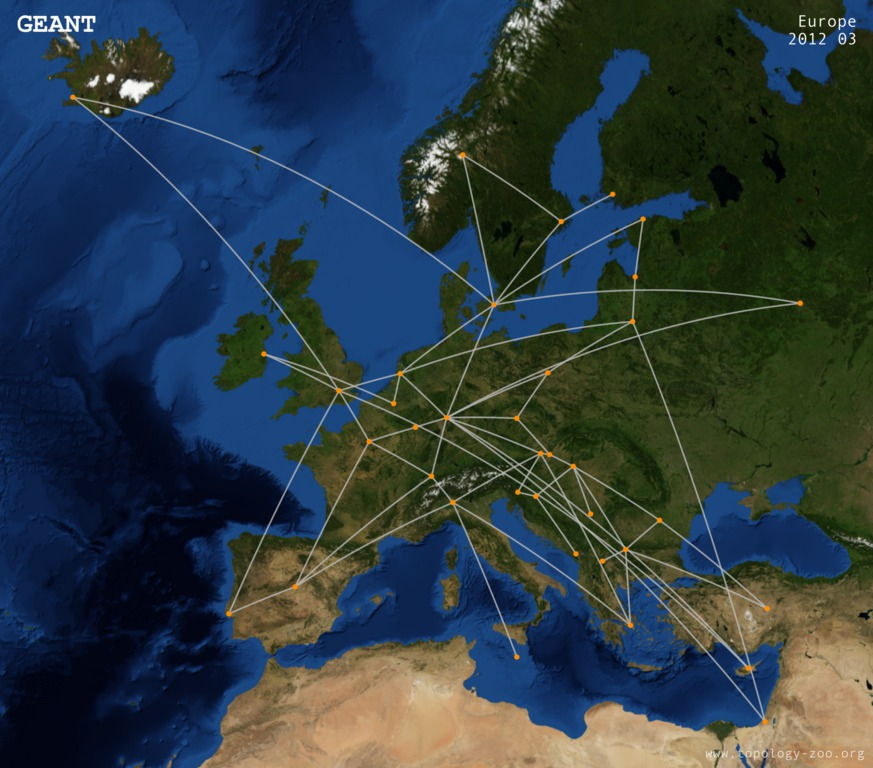
\includegraphics[width=0.7\linewidth]{images/real-world/GEANT_2012.jpg}
    \caption{GEANT (2012) \cite{topology_zoo}}
    \label{fig:GEANT}
\end{subfigure}%
\begin{subfigure}{.5\textwidth}
    \centering
    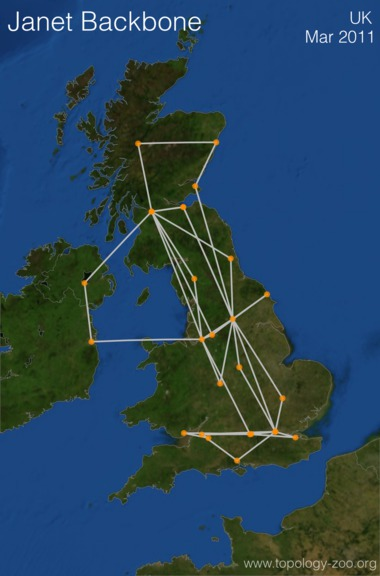
\includegraphics[width=0.5\linewidth]{images/real-world/Janetbackbone_2011.jpg}
    \caption{Janet Backbone (2011) \cite{topology_zoo}}
    \label{fig:janet_backbone}
\end{subfigure}
\caption{Example Backbone primary networks from the Internet Topology Zoo database}
\label{fig:test}
\end{figure}

Topologies are not only visualised but also captured in the GML graph exchange format, enabling straightforward processing of the topologies in a scripting language such as python. 

\begin{figure}
\centering
\begin{subfigure}{.5\textwidth}
    \centering
    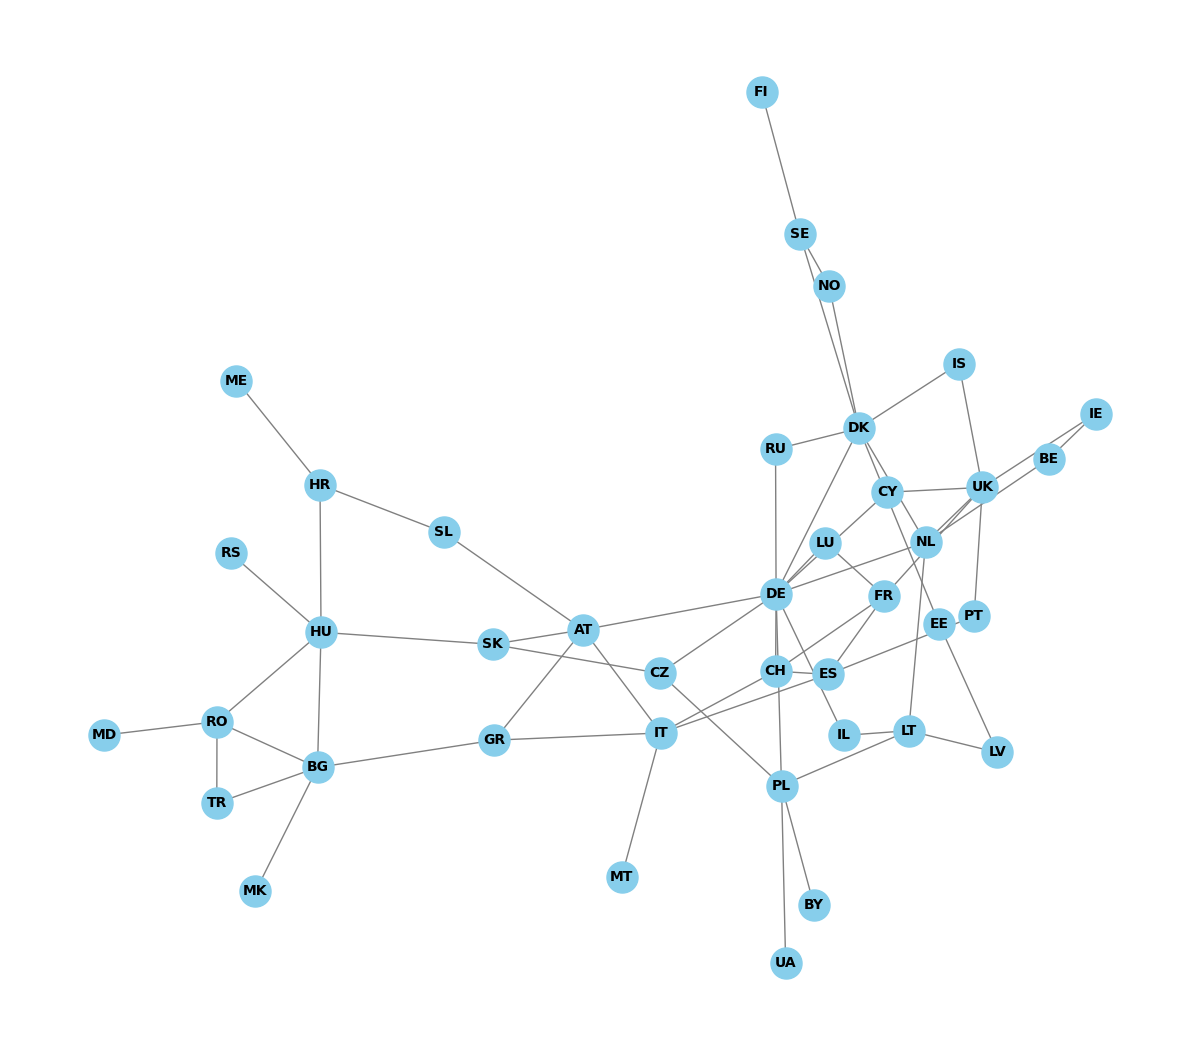
\includegraphics[width=0.7\linewidth]{images/real-world/geant_plot.png}
    \caption{GEANT (2012) \cite{topology_zoo}}
    \label{fig:GEANT_plot}
\end{subfigure}%
\begin{subfigure}{.5\textwidth}
    \centering
    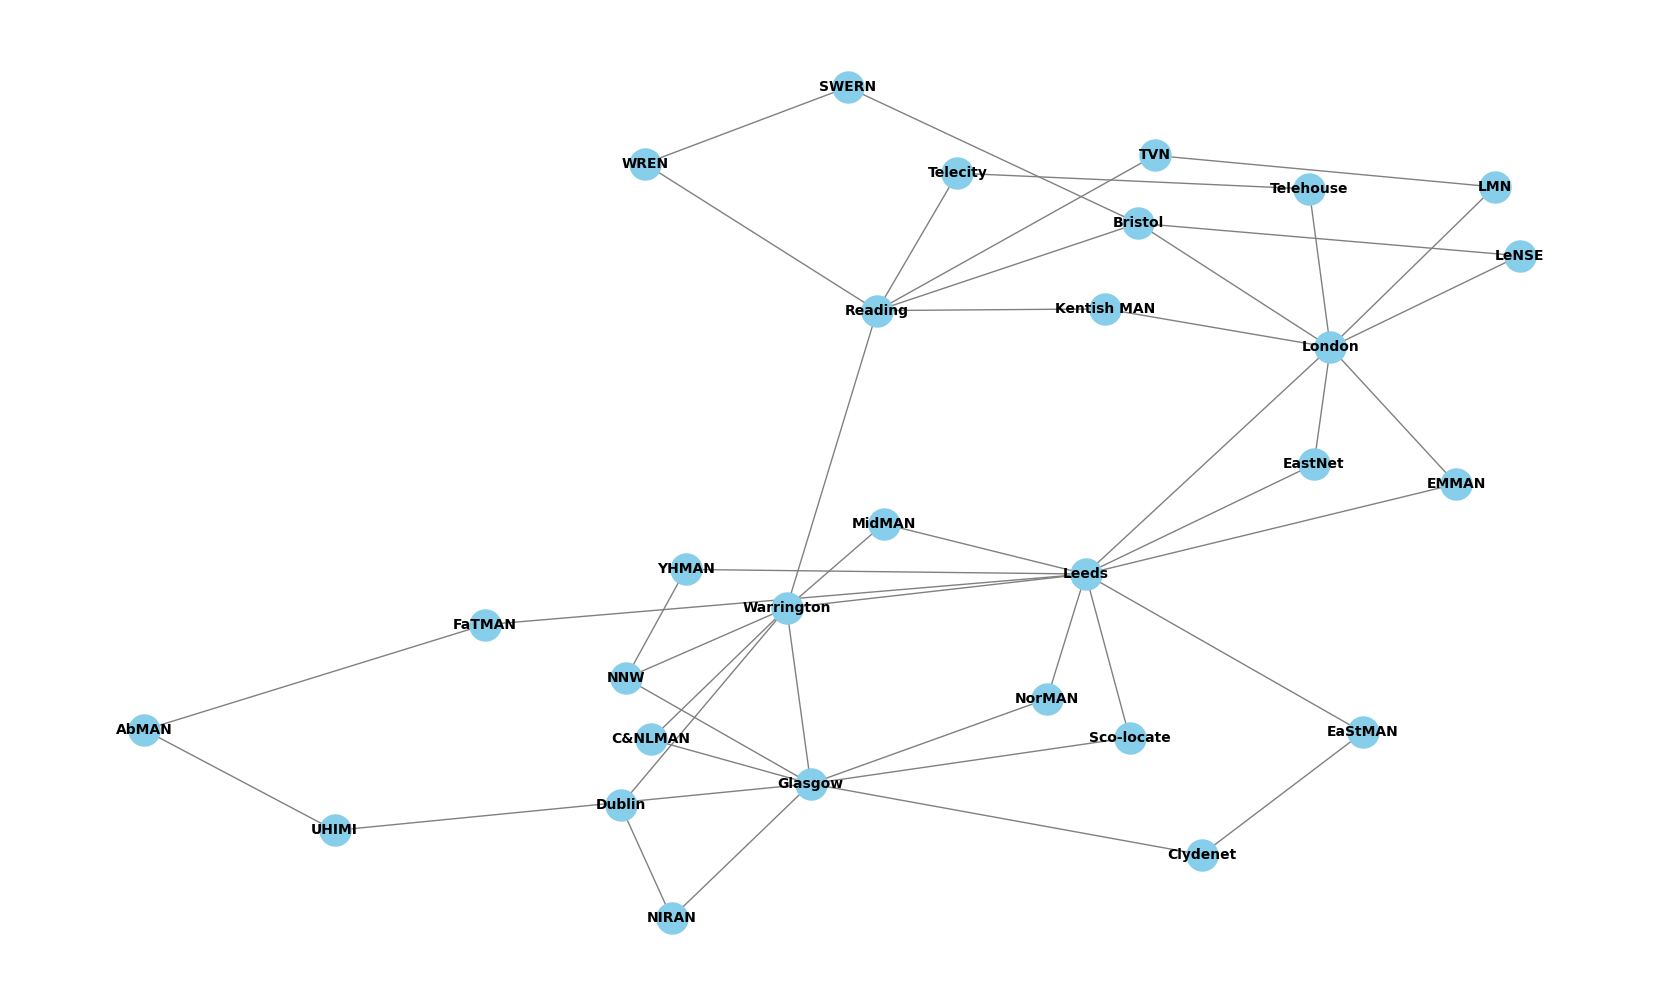
\includegraphics[width=0.7\linewidth]{images/real-world/janet_plot.png}
    \caption{Janet Backbone (2011) \cite{topology_zoo}}
    \label{fig:janet_backbone_plot}
\end{subfigure}
\caption{GEANT and Janet Backbone topologies imported and plotted directly using python}
\label{fig:test}
\end{figure}

By analysing and evaluating contemporary network scanning tools on simulated models of real-world networks, meaningful conclusions can be drawn from experimental results. The practical application of these tools will be tested, in the  environment they were intended to be used for. Furthermore, with a wide variety of different real-world topologies are available through the Internet Topology zoo, extensive and exhaustive testing can be carried out. 

\subsection{Stochastic topologies}
With the aim to implement randomly generated network topologies for the purpose of evaluation in the virtual network lab, several frameworks are discussed below. 
\subsubsection{Parameter definition}
Following an elementary approach which is concerned with the basic 'building-blocks' of a network topology, one can identify these as the number of nodes, the number of links each node has, the origin node and target node of each link. 

\subsubsection{Individual topologies}
Another approach could be to vary the structure of a specific individual topology type at random, based on their defined character and attributes. This would likely be of more interest using more complex structures such as a 'tree' topology, which is expressed through the parameters $d$, $G$.

\subsubsection{Topology library}
A further approach which could be employed would be to have a set of varying basic topologies to form a topology library. This set would include bus, star, mesh and ring topologies of differing sizes and structures. The parameters for random generation of the topology structure in this instance would be the topologies which are to be selected at random from the set, a random number of times, and also how each of these selected topologies would be connected to each other to form a complete logical structure. This approach would have the benefit of being more representative of structures actually found in real-world networks, as opposed to purely random configurations. This is due to being synthesised from component topologies which are actually utilised in the real-world for their individual characteristics.

\begin{figure}
    \centering
    \begin{lstlisting}
import random 

# Individual topology variants
ring = [ring_1, ring_2, ring_3]
bus = [bus_1, bus_2, bus_3]
star = [star_1, star_2, star_3]
mesh = [mesh_1, mesh_2, mesh_3]

# Main topology set
topology_set = [ring, bus, star, mesh]

# Generated topology
generated_topo = []

# Parameter definition
n = 3 # Number of topologies to be selected

for i in range(n):
    # topologies which are to be selected at random from the topology_set, [j,k]
    j = random.randint(len(topology_set)-1)
    k = random.randint(len(topology_set[j])-1)

    # Append to generated topology 
    generated_topo.append(topology_set[j][k])

\end{lstlisting}
    \caption{Example python implementation of random selection from topology library to create new topologies}
    \label{fig:topology_library}
\end{figure}

\subsubsection{Erdos-Renyi Model}
The Erdos-Renyi model \cite{Erdos_renyi_origin} covers two similar mathematical models proposed by Erdos, Renyi and seperately Gilbert \cite{gilbert_background}. They can both be used to randomly generate graphs with a fixed number of nodes $n$. However, the models differ in their approach to creating links between given nodes in the generated graph. The first variant is defined through $G(n,M)$, whereby a graph is generated by randomly selecting one individual instance from the collection of all possible graphs defined by having $n$ nodes and $M$ edges. The random graph selection is uniform, thus each outcome is equally likely to occur. 

\begin{equation}
    G(n,M)
\end{equation}

\begin{algorithm}
\caption{\( G(n, M) \) Erdős-Rényi Model}\label{alg:GnM}
\begin{algorithmic}[1]
\State \textbf{Input:} Number of nodes \( n \), number of edges \( M \)
\State \textbf{Output:} Random graph \( G(V, E) \)

\State \textbf{Step 1:} \textbf{Initialization}
\State Create a set of \( n \) nodes \( V = \{v_1, v_2, \dots, v_n\} \).
\State Initialize an empty set of edges \( E = \emptyset \).

\State \textbf{Step 2:} \textbf{Edge Selection}
\State Let \( \mathcal{P} \) be the set of all possible pairs of nodes \( \{(v_i, v_j) \mid 1 \leq i < j \leq n\} \).
\State Randomly select \( M \) unique pairs from \( \mathcal{P} \) without replacement.

\State \textbf{Step 3:} \textbf{Edge Addition}
\For{each selected pair \( (v_i, v_j) \)}
    \State Add the edge \( (v_i, v_j) \) to the edge set \( E \).
\EndFor

\State \textbf{Step 4:} \textbf{Output the graph}
\State The graph \( G(V, E) \) consists of the node set \( V \) and the edge set \( E \).
\end{algorithmic}
\end{algorithm}

The second variant, proposed by Gilbert is defined through $G(n,p)$, whereby a graph is randomly created by linking labeled nodes in a random manner, according to the parameter $p$ an edge will be added in the graph between two nodes. 

\begin{equation}
    G(n,p)
\end{equation}

\begin{equation}
    p^M(1-p)^{(n \atop 2)-M}
\end{equation}

\begin{algorithm}
\caption{\( G(n, p) \) Erdős-Rényi Model}\label{alg:Gnp}
\begin{algorithmic}[1]
\State \textbf{Input:} Number of nodes \( n \), probability \( p \)
\State \textbf{Output:} Random graph \( G(V, E) \)

\State \textbf{Step 1:} \textbf{Initialization}
\State Create a set of \( n \) nodes \( V = \{v_1, v_2, \dots, v_n\} \).
\State Initialize an empty set of edges \( E = \emptyset \).

\State \textbf{Step 2:} \textbf{Edge Creation}
\For{each pair of nodes \( (v_i, v_j) \) with \( 1 \leq i < j \leq n \)}
    \State Generate a random number \( r \) uniformly distributed between 0 and 1.
    \If{\( r \leq p \)}
        \State Add the edge \( (v_i, v_j) \) to the edge set \( E \).
    \EndIf
\EndFor

\State \textbf{Step 3:} \textbf{Output the graph}
\State The graph \( G(V, E) \) consists of the node set \( V \) and the edge set \( E \).
\end{algorithmic}
\end{algorithm}


A the model is probabilistic, the parameter $p$ exists on the range 0 to 1; intuitively as $p$ increases the likelihood of generating graphs with more links increases, with the converse also being true.

\begin{figure}
    \centering
    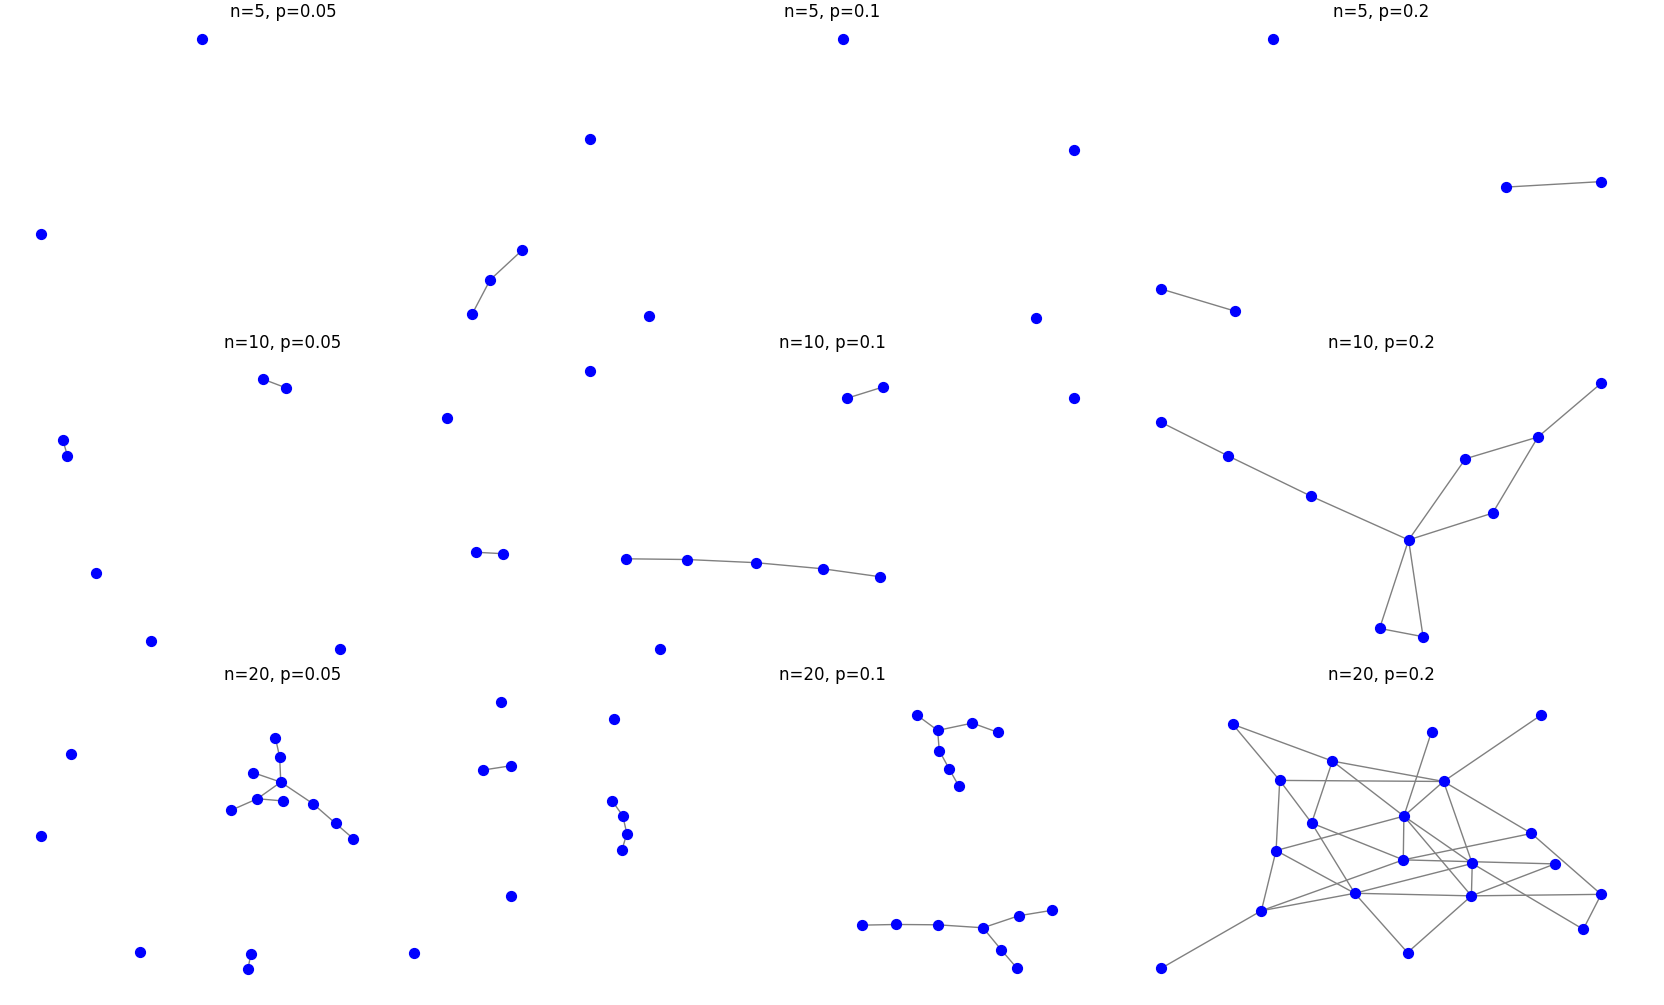
\includegraphics[width=0.75\linewidth]{images/ER/low_prob/low_prob_5,10,20.png}
    \caption{Graph topology plots with varying numbers of nodes, $n$ and probabilities $p$ to illustrate the effect of these parameters on network structure.}
    \label{fig:low_prob_5,10,20}
\end{figure}

\begin{figure}
    \centering
    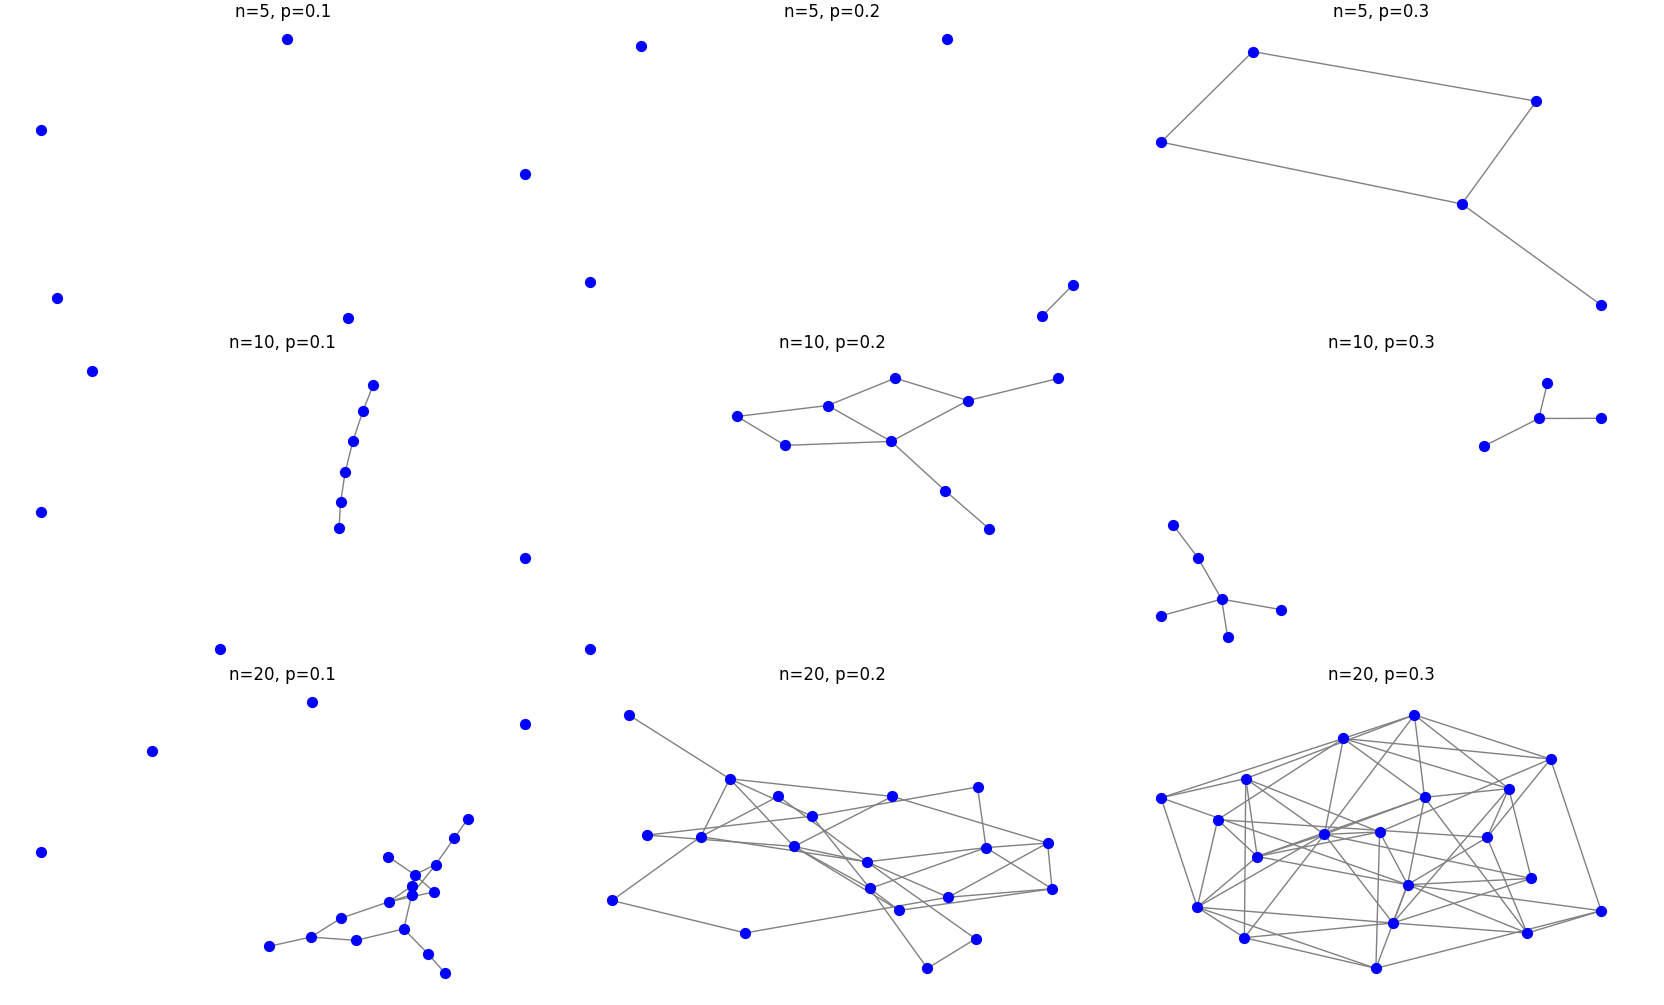
\includegraphics[width=0.75\linewidth]{images/ER/5,10,20.png}
    \caption{Graph topology plots with varying numbers of nodes, $n$ and probabilities $p$ to illustrate the effect of these parameters on network structure.}
    \label{fig:5,10,20}
\end{figure}

\begin{figure}
    \centering
    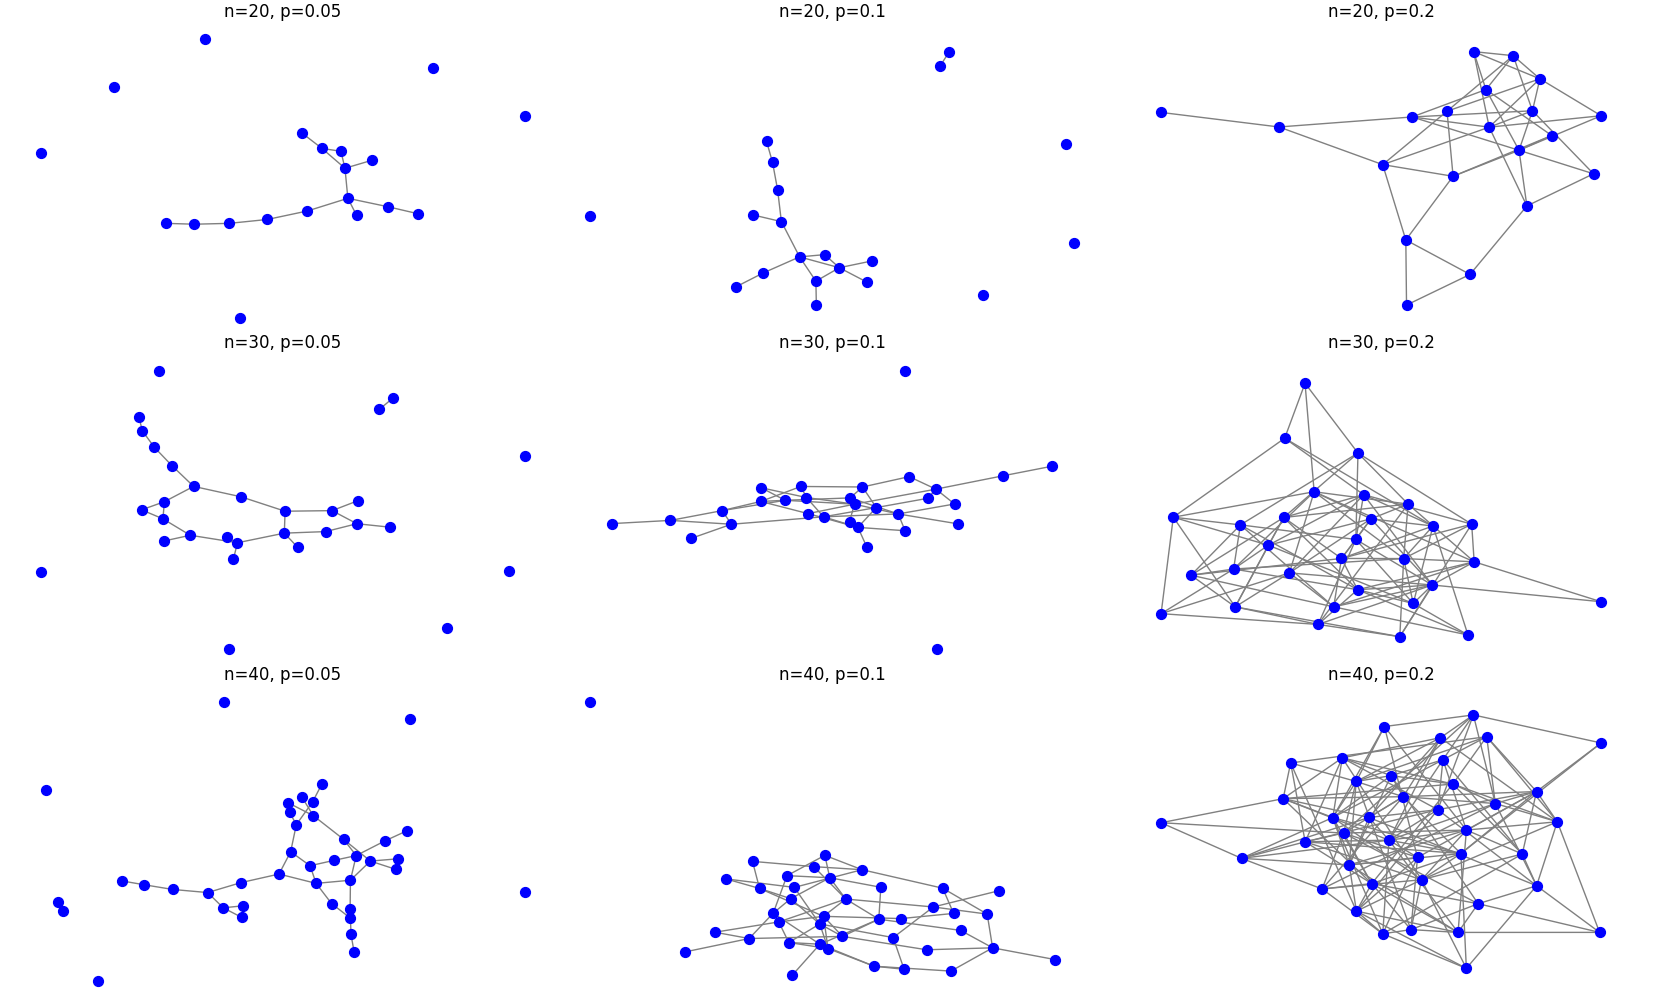
\includegraphics[width=0.75\linewidth]{images/ER/low_prob/low_prob_20,30,40.png}
    \caption{Graph topology plots with varying numbers of nodes, $n$ and probabilities $p$ to illustrate the effect of these parameters on network structure.}
    \label{fig:low_prob_20,30,40}
\end{figure}

\begin{figure}
    \centering
    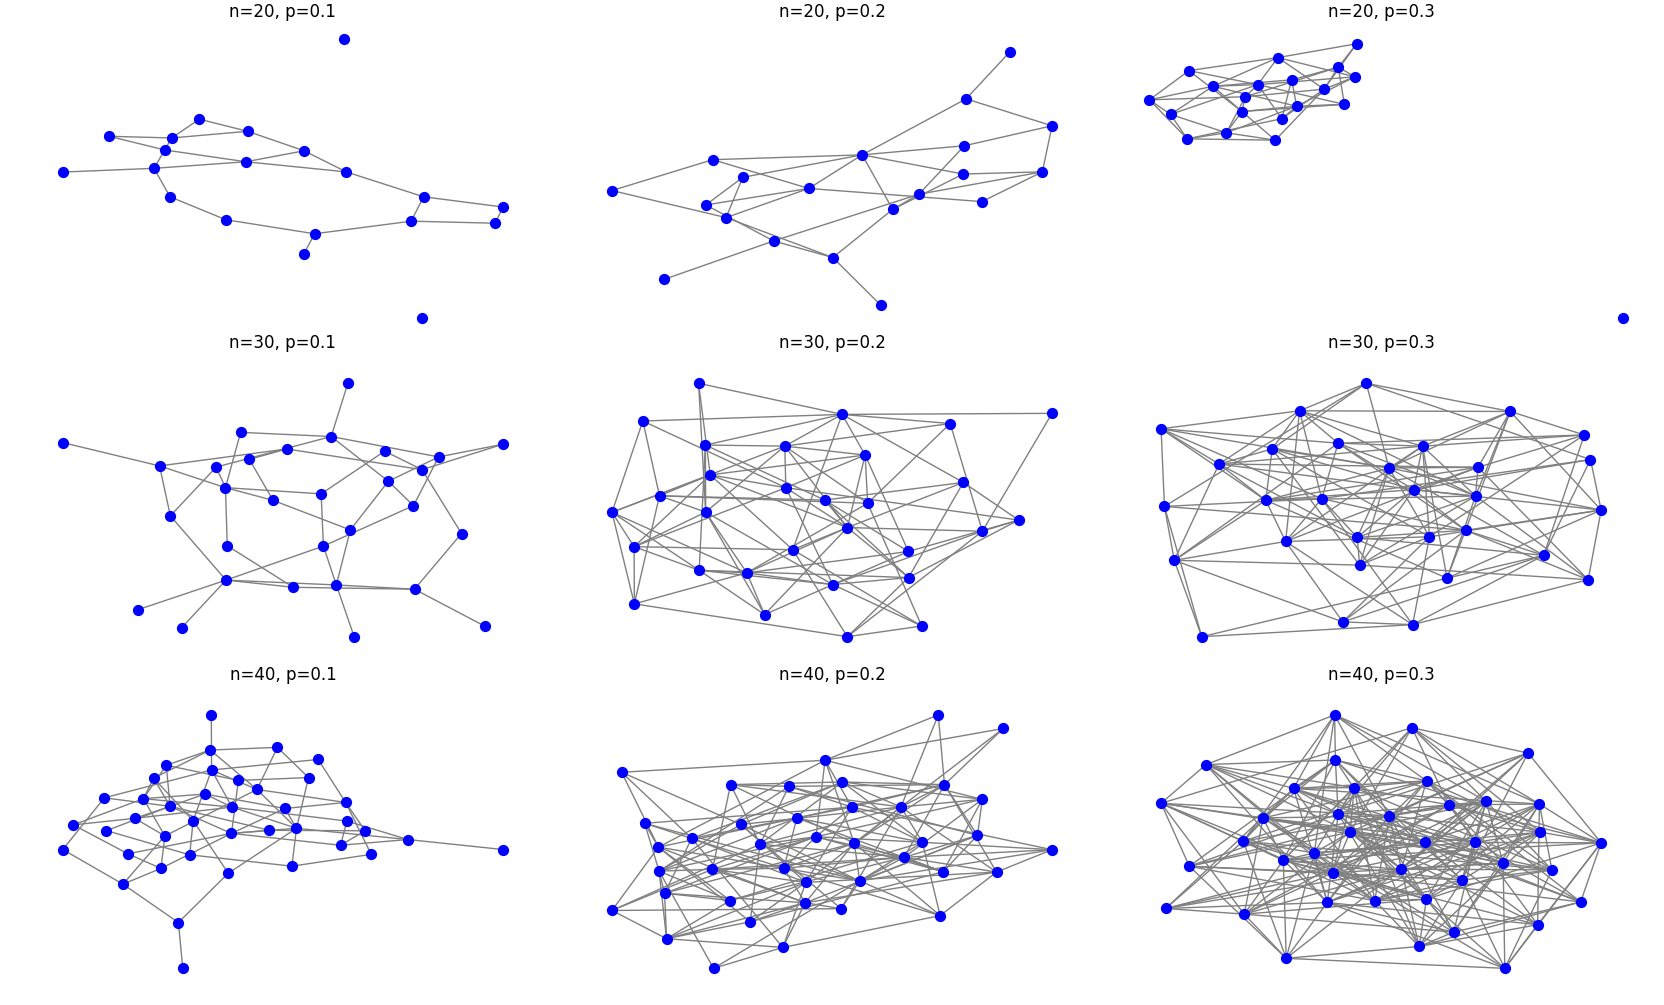
\includegraphics[width=0.75\linewidth]{images/ER/20,30,40.png}
    \caption{Graph topology plots with varying numbers of nodes, $n$ and probabilities $p$ to illustrate the effect of these parameters on network structure.}
    \label{fig:20,30,40}
\end{figure}

For the purposes of network topology generation, the G(n,M) is the seemingly obvious choice between both variants. This is due to every node in the network having at least one link to another node, avoiding unconnected nodes and separated networks. However, ensuring a sufficiently high enough $p$ value, and number of nodes,$n$,  the resultant networks from the $G(n,P)$ model have much more complex structural dynamics and also potential variance across each generated models. It can be argued that this property makes the $G(n,P)$ model preferable to use for evaluation of the network scanning tools, due to the potentially much larger potential diversity of resultant topologies. On the basis of this, the $G(n,P)$ model will be selected for evaluation.

\subsubsection{Barabasi-Albert Model}

%Discuss how it is likened to real-world networks such as the WWW and social networks, think it would be highly applicable for this use-case.
The Barabasi-Albert model is an algorithm which  produces random scale-free networks. The networks are generated utilising a preferential attachment approach, whereby the more links a given node has to other nodes, the higher the probability it will get more new links. A node's degree corresponds to the number of links it has to other nodes, therefore the higher the degree a node has, the higher the probability of garnering new link's with other nodes it has. 

Initially the network starts with a network of $m_0$ nodes, at each step a new node is added with $m$ edges which link it to $m$ different nodes. The probability that a new node will connect to an existing node $i$ is given by \ref{eq:3}, where $k_i$ is the degree of node $i$, and the sum is over all existing nodes $j$. \cite{Albert_barabasi_2002} 

\begin{equation} \label{eq:3}
    p_i = \frac{k_i}{\Sigma_jk_j}
\end{equation}

As a consequence of this, the higher the number of links that a node has in a topology generated through the Barabasi-Albert method, the higher the likelihood that that same node will receive more new links. The same pattern occurs across many different real-world networks, such as the world wide web and social networks; whereby well-known websites and people which are both highly connected are more likely to be connected to a new website or person than a less connected person or website.  

\begin{figure}
    \centering
    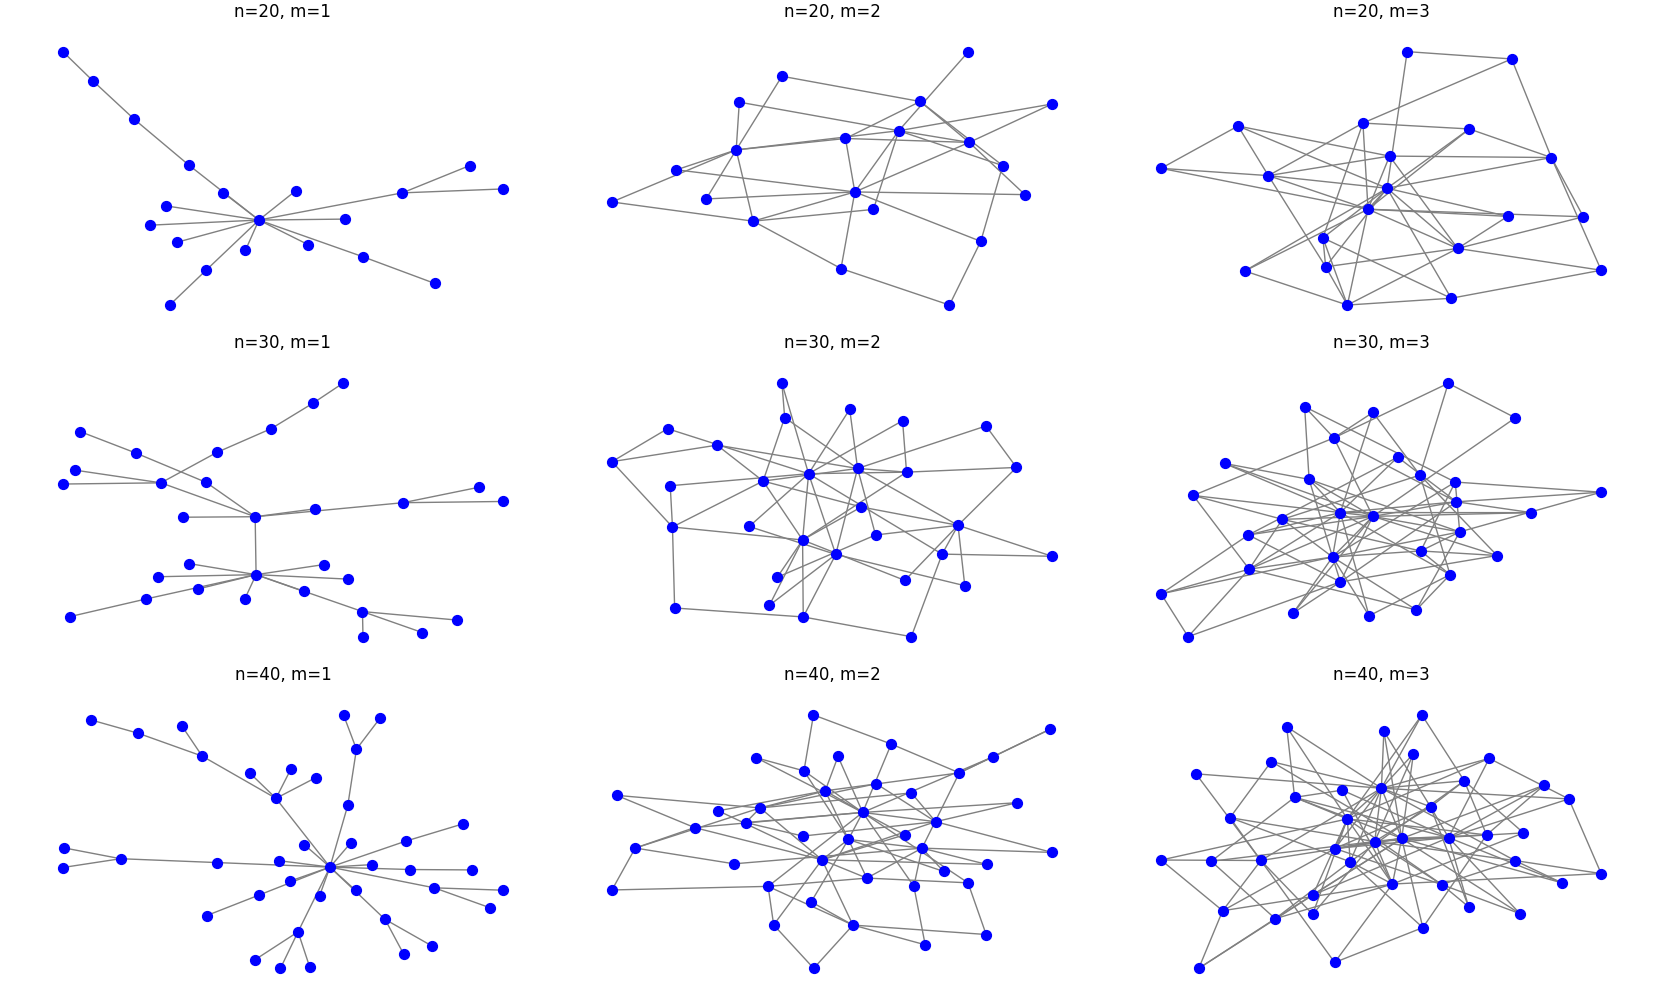
\includegraphics[width=0.75\linewidth]{images/BA_9.png}
    \caption{9 different randomly generated networks using the BA model algorithm, each with varying n and m values to illustrate the impact of each parameter}
    \label{fig:BA_9}
\end{figure}


\subsubsection{Python Implementation}
Each of these approaches could be facilitated by implementing them in python to create custom topology definition files in such a way which can then be parsed by containerlab to deploy and host the topologies virtually. 
The python library networkx \cite{networkX} has stochastic graph generating functions which can implement the Erdos-Renyl and Barabasi-Albert models, reducing overall development time and ensuring accurate and efficient code. 

\subsection{Generated and Real-world Topologies comparison}
To investigate the difference between methods used to generate the stochastic topologies in the context of real-world networks, they will be compared with the real-world topologies found from the Internet Topology Zoo database using the distribution of the shortest path length and also their degree correlation coefficient to ensure a rigorous and comprehensive approach.


The results of this comparison are to be used as the basis of selection from the different topology generation methods mentioned previously, with the most closely correlated models being recommended to be used in the implementation of the final network topologies in the proposed virtual network lab. 

However, in order to provide ample variance and a larger testing area, generated models which are not closely correlated to ones found in real-world topologies are also of great utility. By providing potentially novel testing environments and structures, network scanning tools and otherwise can be more thoroughly evaluated; providing richer data. It is not clear how to strictly evaluate how 'novel' a given model is, although by differing from real-world and other topology generation method it could be argued that would be a suitable basis on which to suggest novelty/uniqueness of topology.

\subsubsection{Distribution of shortest path lengths}
The shortest path length is concerned with the shortest possible path between two given nodes, denoted $i$ and $j$.  By examining the distribution of each of these lengths between every node in a given topology, the distribution of shortest path lengths can be revealed. 

It can be mathematically defined using notation from graph theory; the shortest path length of a given graph $G = (V,E)$ which represents a topology, where $V$ is the set of $|V|=N$ nodes and $E$ is the set of $|E|=M$ edges, is defined as "The number of edges on the shortest path from i to j is the shortest path length ($s'$) of that path. The $s'$ is a number associated with the pair $i-j$: for each pair $i-j$ there is one and only one $s':s'(i,j)$"\cite{santos2022shortestpathpathlength} \cite{DSPL_second_source}

\subsubsection{Degree Correlation Coefficient}
The second metric used to compare the varying network topologies is their Degree correlation. It is defined as:
"[capturing] the relationship between the degrees of nodes that link each other" \cite{barabasi2016network} This measurement reflects the modality of how a given networks nodes link together, due to the degree comparison between two given nodes. 

\begin{equation}
    k_{nn}(K_i) = \frac{1}{K_i}\sum^{N}_{J=1}A_{ij}k_j
\end{equation}

A nodes degree is a measure of being how many connections it has with other nodes in a network. Highly connected nodes have a high degree and are also sometimes known as "hubs". Due to a phenomenon known as the "Friendship paradox", nodes are more likely to be linked to other nodes which have a higher degree(hubs) than nodes with a smaller degree. However, not all networks conform to this trend, with network types being characterised in the context of degree correlation as either neutral, assortative or disassortative. Neutral networks are interconnected at random, assortative networks operate according to the friendship paradox whereby hubs tend to connect to other hubs, and lastly disassortative networks, whereby hubs tend not to connect to one another in favour of small degree nodes. 

\begin{figure}
    \centering
    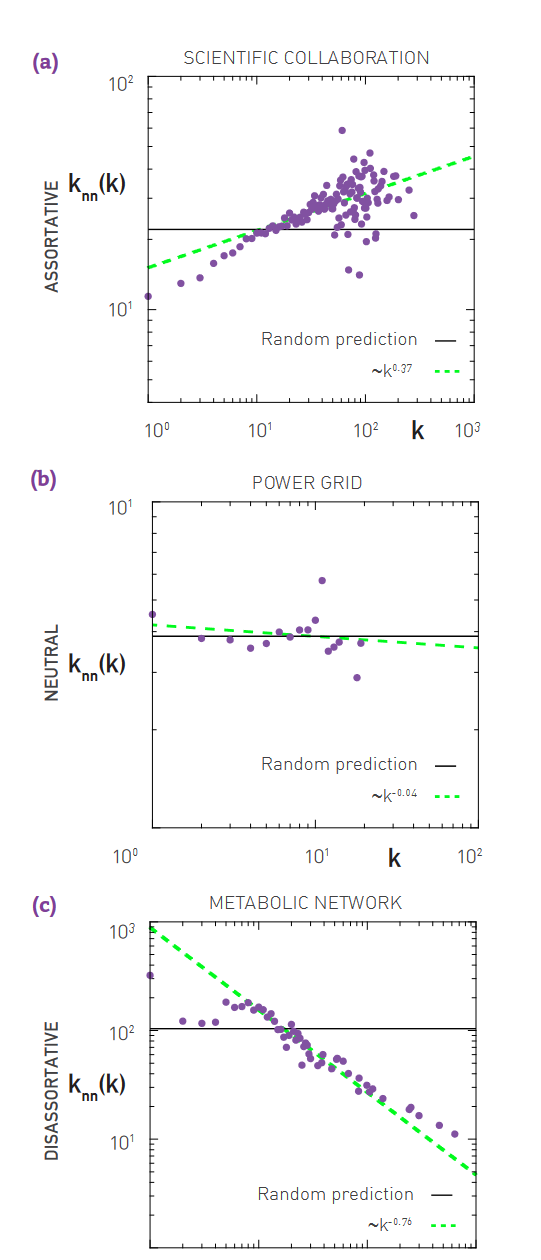
\includegraphics[width=0.3\linewidth]{images/Degree_Correlation_Examples.png}
    \caption{Real world examples of Assortative, Neutral and Dissassortative networks \cite{barabasi2016network}}
    \label{fig:Example_Degree_Corr}
\end{figure}

In other words, the Degree correlation of a given network can characterise whether a network is neutral, assortative or disassortative. The degree correlation coefficient \cite{Assortive_Mixing} can be used to distinguish individual network degree correlations as a single number. Which is useful for comparison across multiple networks. It is defined through the following equation:

\begin{equation}
    r= \sum_{jk}\frac{jk(e_{jk}-q_jq_k)}{\sigma^2}
\end{equation}

with,

\begin{equation}
    \sigma^2 = \sum_{k}k^2q_k-\left[\sum_{k}kq_k\right]^2
\end{equation}

$r$ is the Pearson correlation coefficient between the degree of each node across their shared link. \cite{barabasi2016network} It exists on the range between $-1 <=r<=1$, with assortative networks resulting in $r<0$, $r=0$ for neutral networks and $r>0$ for disassortative networks. 

%compare the generated networks and real-world networks r value, as a measure of correlation and therefore relavance in testing the network scanning tools


\subsection{Virtual Lab implementation}

\subsubsection{Oracle VM VirtualBox}
% Virtual environment allows greater portability
Oracle VM VirtualBox is an open source cross-platform virtualization software using a Type 2 hypervisor. \cite{VirtualWare} It's ease of installation and use on all of the major Operating Systems including Microsoft Windows, macOS, Linux, Solaris and OpenSolaris \cite{oracleVM} allows for high portability and cohesion. 

Due to the traceroute tools being developed for a Linux based operating system, VirtualBox is being used to host a Linux distribution on a windows machine without the need for a dual-boot or separate computer.

\subsubsection{Docker}
% Outline docker, and containers
Docker allows application images to be deployed in isolated containers \cite{docker_isolate}. This avoids the potential computational overhead of running an operating system using a virtual machine, and also allows for ease of deployment. It can be built into new and existing pipelines for automatic CI/CD, which is particularly advantageous in industry contexts. 

\subsubsection{ContainerLab}

% Outline containerlab, various topologies employed
ContainerLab builds upon the containerisation technology which docker provides. It centers on Network Operating Systems which are commonly used commercially and for network testing and diagnostics. This provides a more realistic testing environment which reflects real-world networks. Furthermore, it also allows a wide range of possible configurations between multiple different nodes running different Network Operating Systems.

\begin{figure}
    \centering
    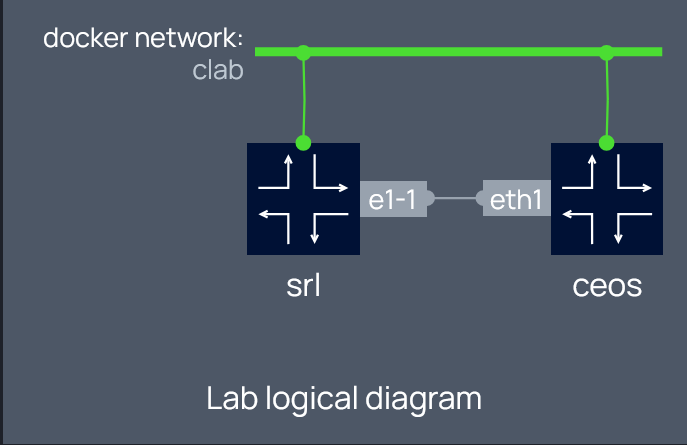
\includegraphics[width=0.5\linewidth]{images/lab_logical_diagram.png}
    \caption{Example Lab logical diagram \cite{containerlab}}
    \label{fig:lab_diagram_example}
\end{figure}

Configuration and management is controlled through a command-line interface (CLI), with the virtual topologies being defined straightforwardly in human readable YAML format. The topology is defined as "a set of nodes and links between them" \cite{containerlab}. Each of the nodes contains a kind to specify/control node behaviour, additionally each node also has an image link to the Network Operating System image to be loaded. The structure of the network is determined through a set of endpoints, expressing how each node is connected.

\begin{figure}
    \centering
    \begin{lstlisting}
name: srlceos01

topology:
  nodes:
    srl:
      kind: nokia_srlinux
      image: ghcr.io/nokia/srlinux
    ceos:
      kind: arista_ceos
      image: ceos:4.32.0F

  links:
    - endpoints: ["srl:e1-1", "ceos:eth1"]
\end{lstlisting}
    \caption{Example ContainerLab network topology defined in YAML file}
    \label{fig:topology_yml}
\end{figure}

Upon deployment of the lab, the lifecycle can be managed through deploy, destroy, save, inspect and graph operations. Further increasing it's utilitiy and usability as a virtual network lab.

\begin{figure}
    \centering
    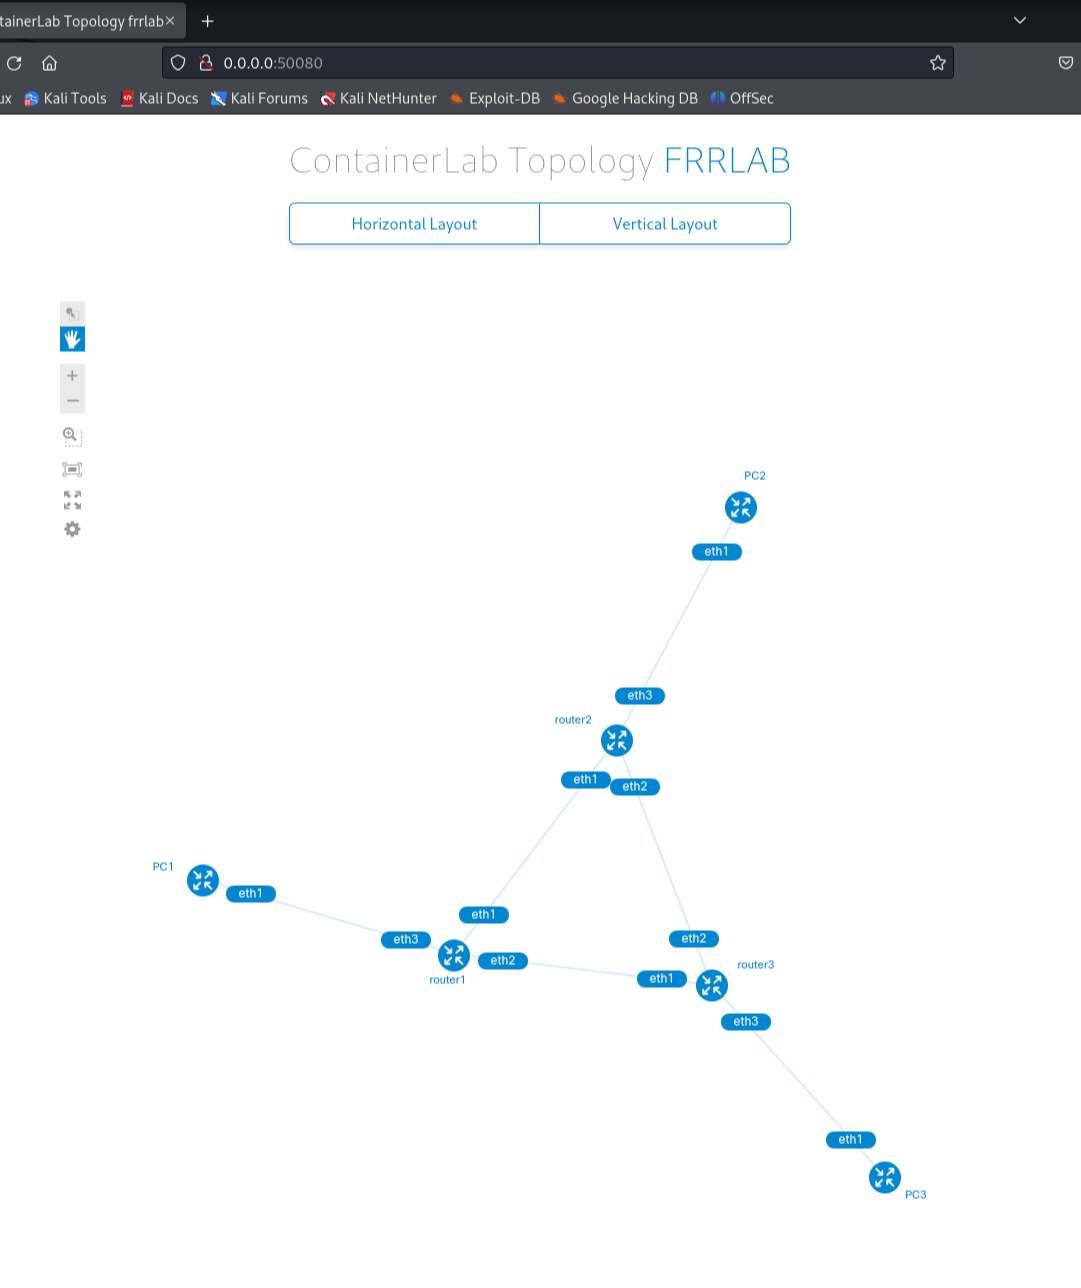
\includegraphics[width=0.5\linewidth]{images/ring_containerlab.png}
    \caption{Containerlab network topology visualisation feature, showing a simple ring network structure.}
    \label{fig:ring_container}
\end{figure}

\subsubsection{Alpine Linux}
% Lightweight distro
For the implemented virtual network lab, Alpine Linux has been used due to it's small size and resource efficiency. When installed on a container, it  requires a minimal 8 MB of space \cite{alpine}. However, this reduction of space overhead has a trade-off; an instance of this is that Apline uses a non-regular package manager called apk; this has proved to be problematic during creation of the network lab, due to lack of support to install the required network scanning libraries on containers to facilitate testing. 

\subsubsection{NetworkX}
%Describe framework
NetworkX is a python library which is designed to be used for the "creation, manipulation, and study of the structure dynamics, and functions of complex networks." \cite{networkX} Due to it's extensive functionality, utilising this library for the evaluation and processing of graph topologies increases the speed and ease with which it can be carried out. Furthermore, as a consequence of it's robust implementation and over 90\% test coverage of it's code-base, results yielded from code utilising this library are highly trustworthy. 

%Modules used from framework
For the generation of random graph topologies, namely Erdos-Renyi and Barabasi-Albert, the corresponding modules are used; \newline
\verb|erdos_renyi_graph(n, p, seed=None, directed=False)| 
\verb|barabasi_albert_graph(n, m, seed=None, initial_graph=None)| 

For the comparison between the various topologies the following modules were used; \newline 
\verb|all_pairs_shortest_path_length(G, cutoff=None)|
%Code excerpt

\subsubsection{Virtual network pipeline}
As previously mentioned, to facilitate simulation of the randomly generated network topologies, the generated structures could be parsed into the YAML format required for containerlab to deploy virtual networks. Implementation of a seamless "pipeline" is of great benefit as it allows modular steps in the creation of the network lab to be connected linearly, allowing straightforward configuration and control of each step in the process. Furthermore, it also has the additional benefit of being more extensible and resilient to bugs and anomalies as these can be isolated at specific stages in the pipeline. An additional benefit is ease of use, should the framework be adopted in the future for further research. Below, a framework is proposed with the aim of accomplishing this; from the initial generation of network topologies to the simulation and evaluation of them using configurable contemporary methods. 

\begin{figure}
    \centering
    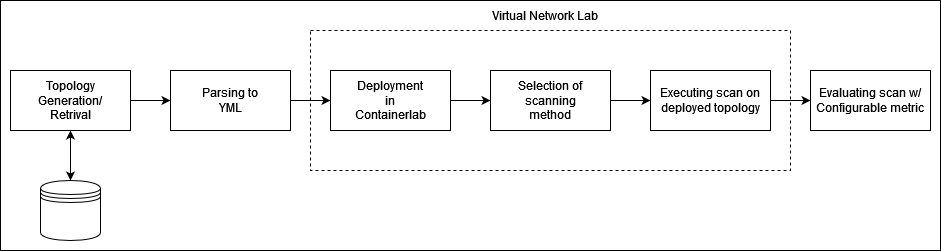
\includegraphics[width=0.9\linewidth]{images/topo_pipeline.png}
    \caption{Diagram illustrating proposed topology deployment and evaluation pipeline}
    \label{fig:topo_pipe}
\end{figure}

topology generation $\Rightarrow$ parsing to YML $\Rightarrow$ deployment of containerlab environment $\Rightarrow$ selection of network scanning method $\Rightarrow$ running scan on deployed topology $\Rightarrow$ evaluating scan using configurable metric 

To facilitate simulation of real-world topologies from the Internet Topology Zoo dataset, a similar pipeline is proposed. In which the GML graph files are parsed to YML format, which are then deployed using containerlab, continuing onto be scanned using a chosen scanning method and evaluated using a configurable metric.  

Topology selection from Dataset $\Rightarrow$ parsing to YML $\Rightarrow$ deployment of containerlab environment $\Rightarrow$ Selection of scanning method $\Rightarrow$ running scan on deployed topology $\Rightarrow$ evaluating scan using configurable metric 

% Create diagrams for each step in pipeline, with accomanying code to go with each step. 

\begin{figure}
    \centering
    \begin{lstlisting}
#Parse to YML 
def parse_to_yml(graph : nx.graph, image, kind):

    #Define output file name
    output_file = "output_topology.yaml"

    #Define topology as a dictionary
    topology = OrderedDict({
        "name": "output_topology",
        "topology": OrderedDict({
            "nodes": OrderedDict(),
            "links": []
        })
    })

    #Adding definitions to each node in topology
    for node,i in enumerate(graph.nodes):
        topology["topology"]["nodes"][f"node{node}"] = {
            "kind" : kind,
            "image" : image,
        } 

        #Creating links between the nodes
    for edge in graph.edges:
        topology["topology"]["links"].append({
            "endpoints" : [f"node{edge[0]}:eth1", f"node{edge[1]}:eth1"]
        })

    #Parse topology to YAML file
    with open(output_file, 'w') as yaml_file:
        yaml.dump(topology, yaml_file, default_flow_style=False)


\end{lstlisting}
    \caption{Python function to parse graph topology to YAML file which can be read by containerlab and used to deploy simulated virtual network topology}
    \label{fig:python_parse_function}
\end{figure}

\begin{figure}
    \centering
    \begin{lstlisting}
name: output_topology
topology:
  nodes:
    node0:
      image: ghcr.io/nokia/srlinux
      kind: srl
    node1:
      image: ghcr.io/nokia/srlinux
      kind: srl
    node2:
      image: ghcr.io/nokia/srlinux
      kind: srl
    node3:
      image: ghcr.io/nokia/srlinux
      kind: srl
  links:
  - endpoints:
    - node0:eth1
    - node1:eth1
  - endpoints:
    - node0:eth1
    - node2:eth1
  - endpoints:
    - node0:eth1
    - node3:eth1
  - endpoints:
    - node1:eth1
    - node3:eth1
\end{lstlisting}
    \caption{Example resultant YAML file using python parsing function}
    \label{fig:parse_topo_example_yml}
\end{figure}

\newpage

\subsubsection{Proposed topologies}
Six sets of three topologies are proposed to be evaluated, the selected topologies include randomly generated and real-world topologies. Each set has network topologies of varying size and parameters; this is with the aim to achieve a balanced testing environment, with sufficient variance and provide a diverse range of structures which could be utilised in an experimentation context. The randomly generated topologies have been generated using the Erdos-Renyi and Barabasi-Albert method, and the real-world topologies have been selected from the Internet Topology Zoo database. 

This approach does have limitations however, including selection bias, and a relatively small number of test-cases. By utilising the previously mentioned virtual network pipeline, which would automate the testing process, one could increase the number of tested topologies and address these limitations. Furthermore, some of the network topologies which are proposed to be used for the virtual network lab have a large size and complexity, which could be unfeasible to implement and simulated due to resource constraints. 
This is a further limitation, as it restricts the size and complexity of the final proposed topology models; the network scanning tools are often used to scan large, complex networks where the structure is unknown, which this virtual network lab is unable to replicate. However, given suitably increased resources, the proposed framework and testing environment could support vastly larger networks with greater complexity to address this limitation. 

\begin{figure}
    \centering
    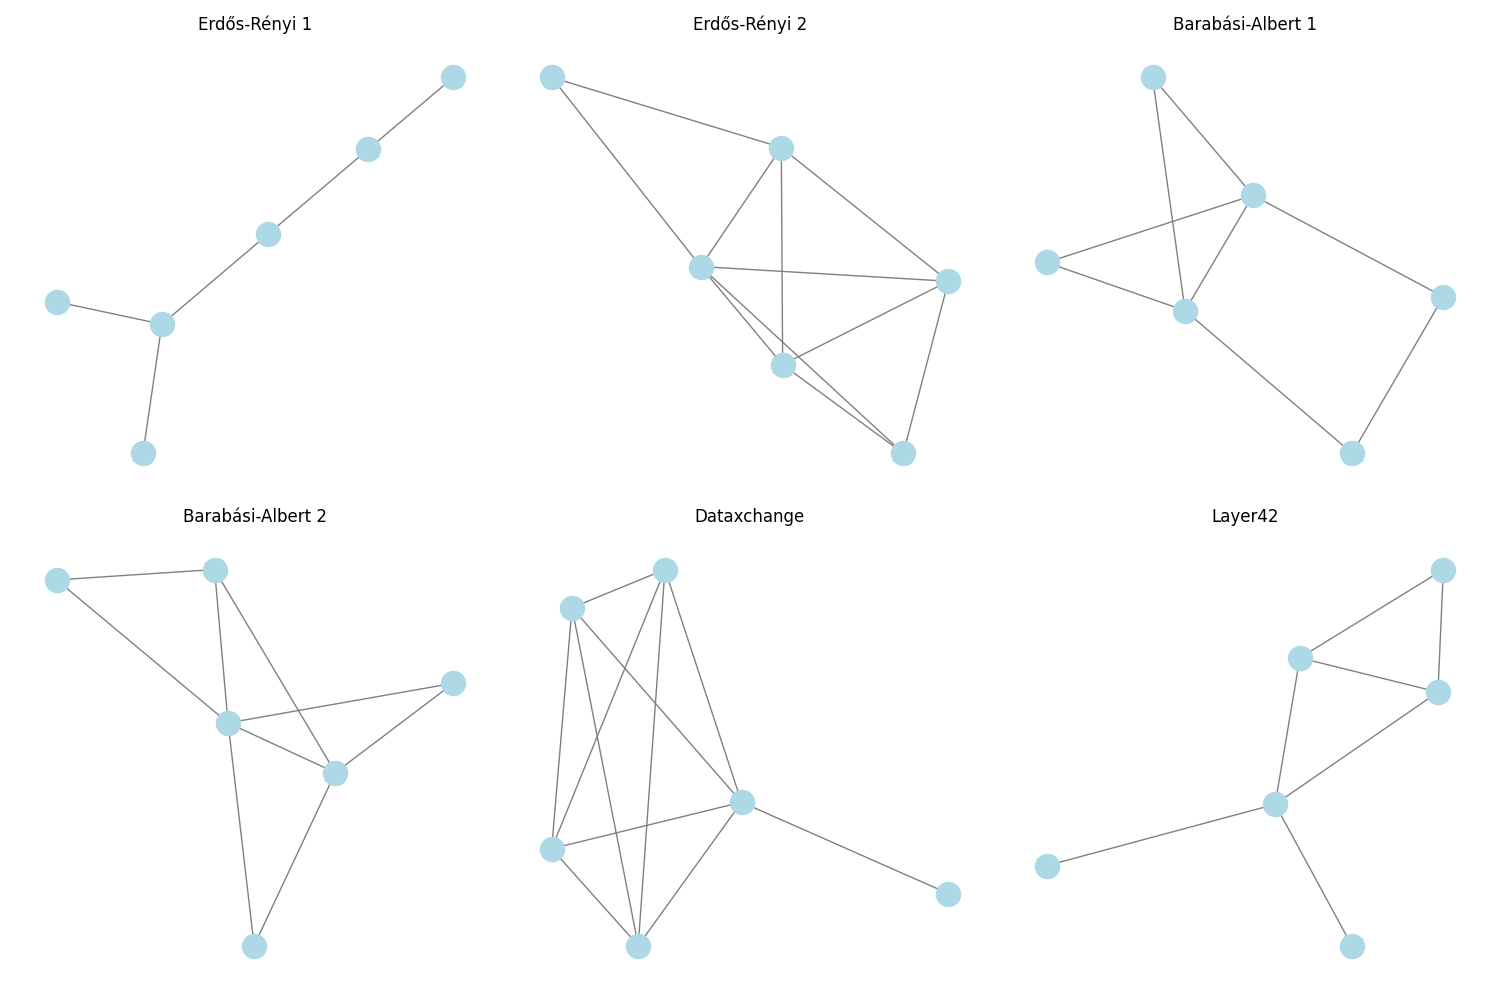
\includegraphics[width=0.8\linewidth]{images/Topology set/6.png}
    \caption{Proposed topologies (6 Nodes)}
    \label{fig:6_prop}
\end{figure}

\begin{figure}
    \centering
    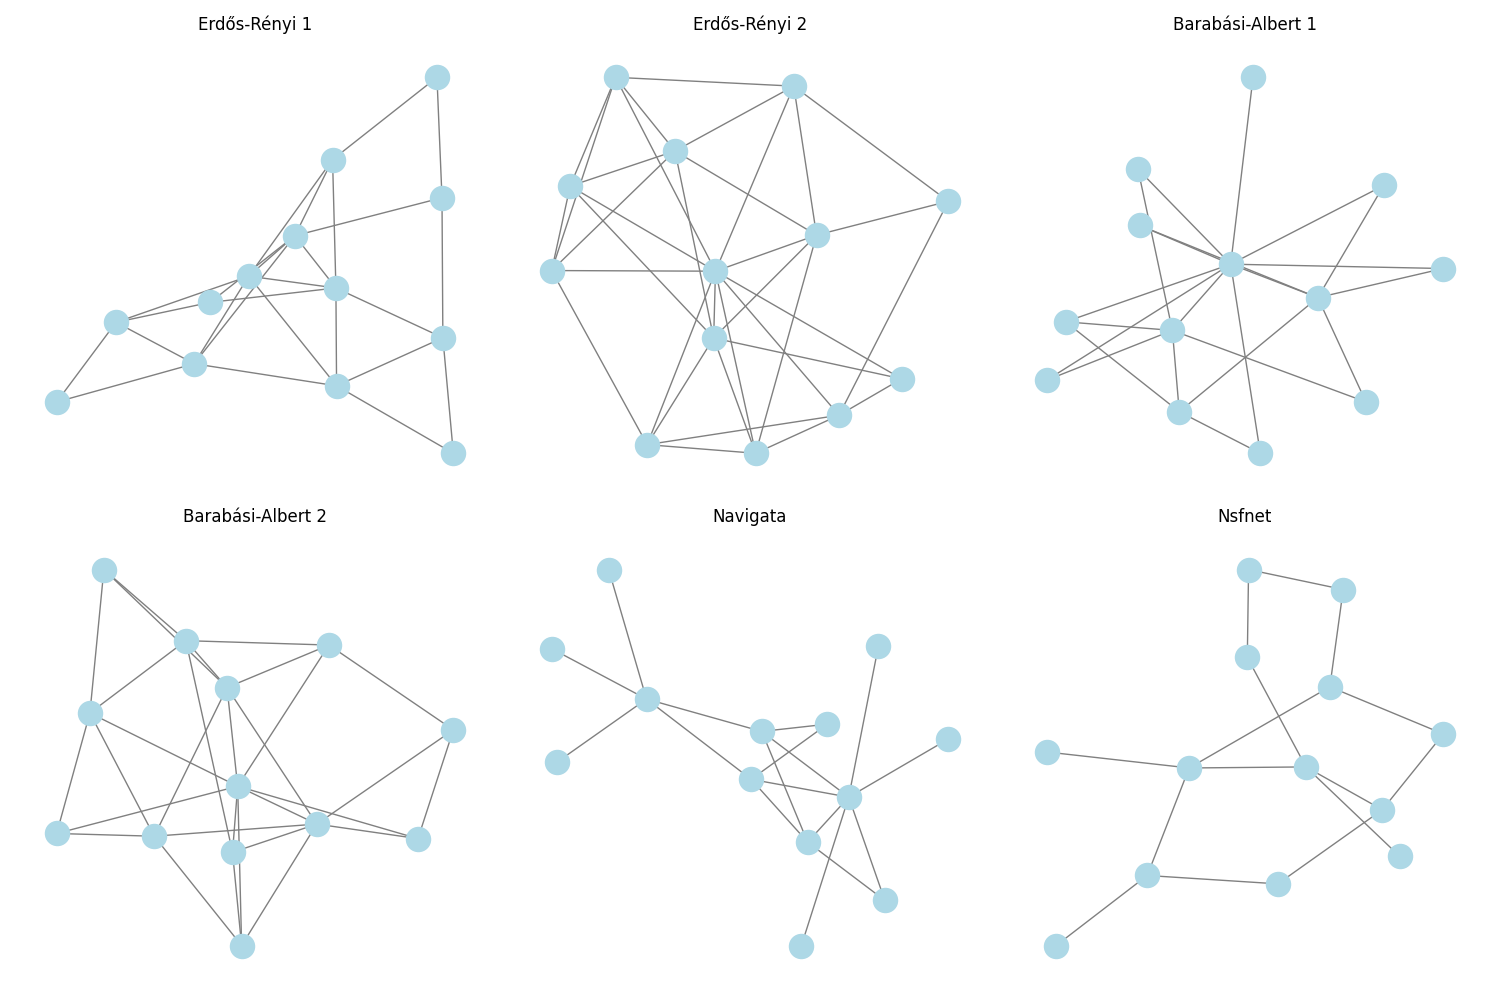
\includegraphics[width=0.8\linewidth]{images/Topology set/13.png}
    \caption{Proposed topologies (13 nodes)}
    \label{fig:13_prop}
\end{figure}

\begin{figure}
    \centering
    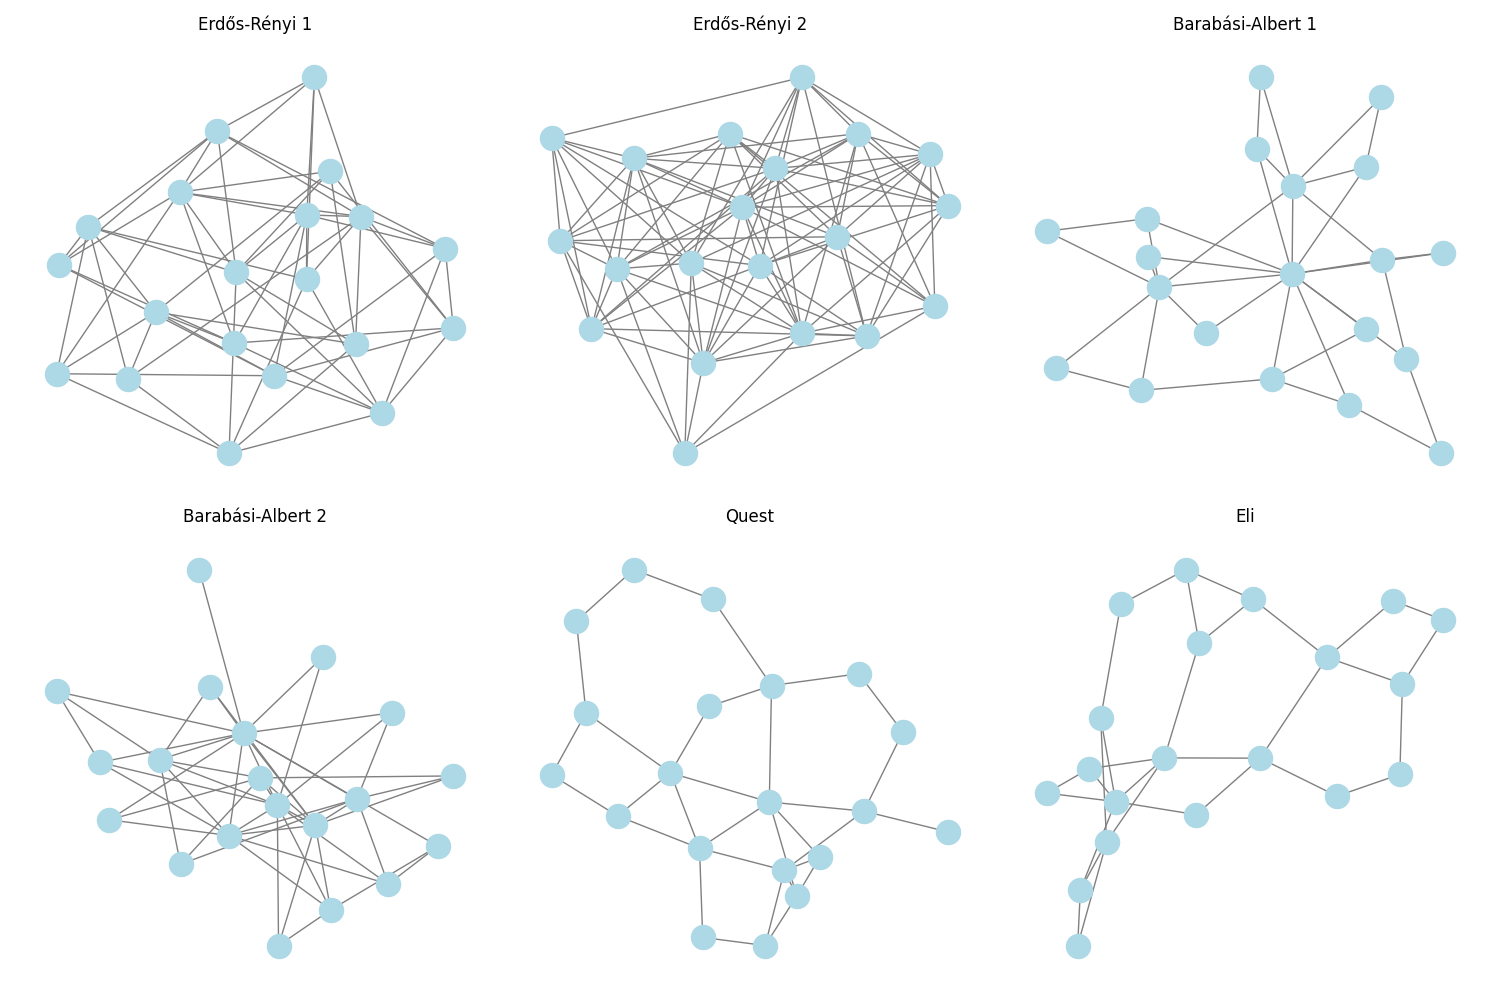
\includegraphics[width=0.8\linewidth]{images/Topology set/20.png}
    \caption{Proposed topologies (20 nodes)}
    \label{fig:20_prop}
\end{figure}

\begin{figure}
    \centering
    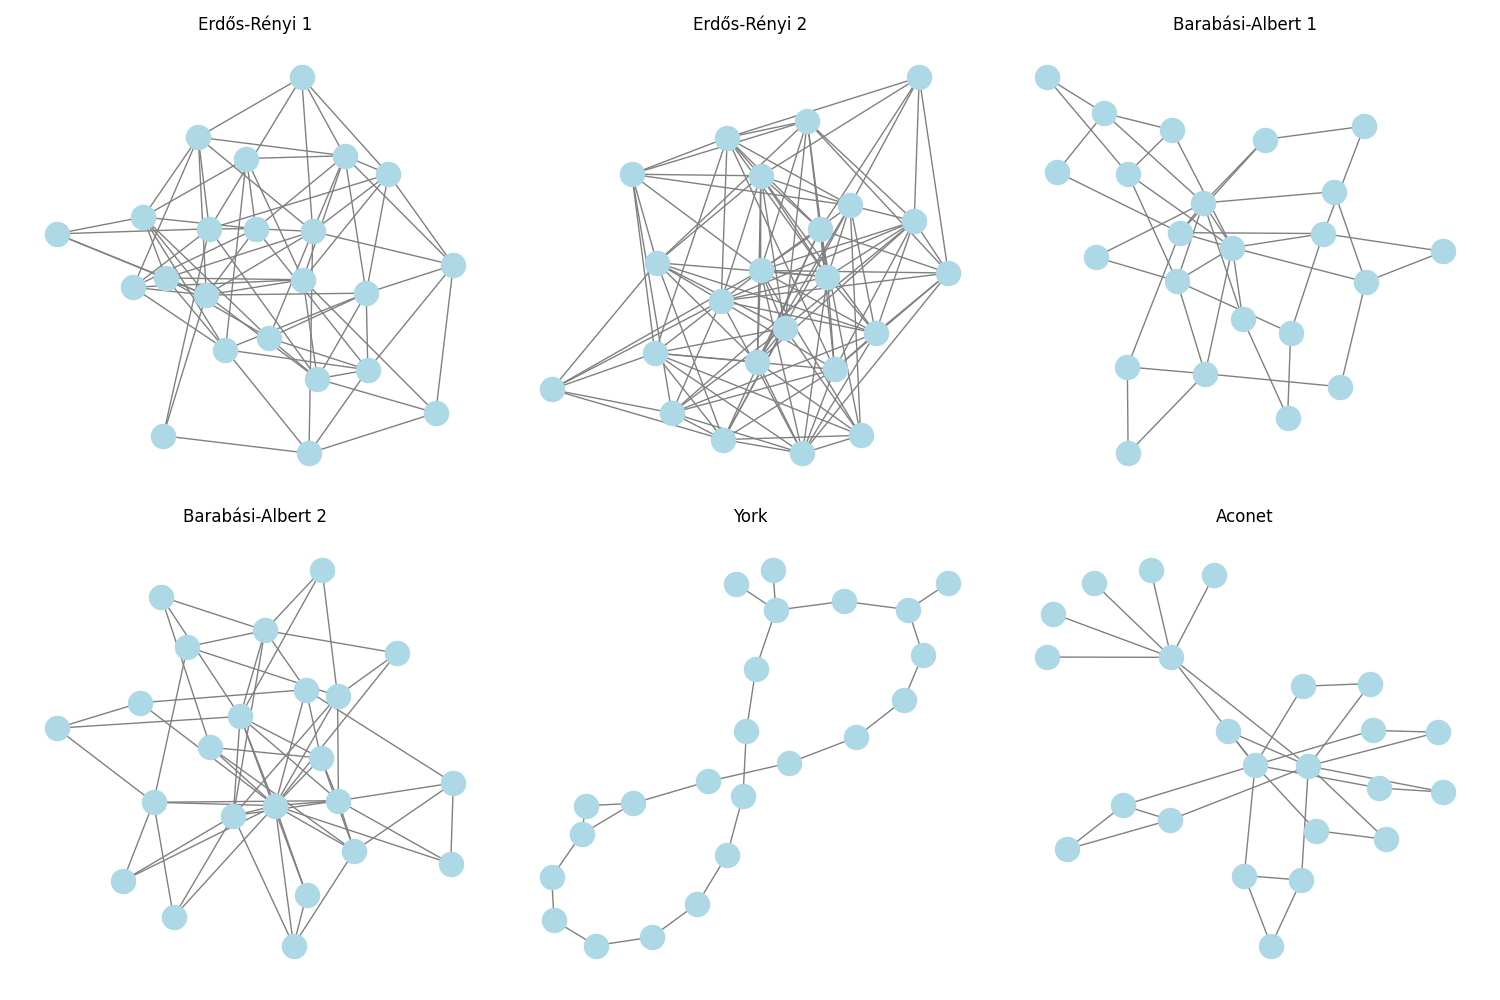
\includegraphics[width=0.8\linewidth]{images/Topology set/23.png}
    \caption{Proposed topologies (23 nodes)}
    \label{fig:23_prop}
\end{figure}

\begin{figure}
    \centering
    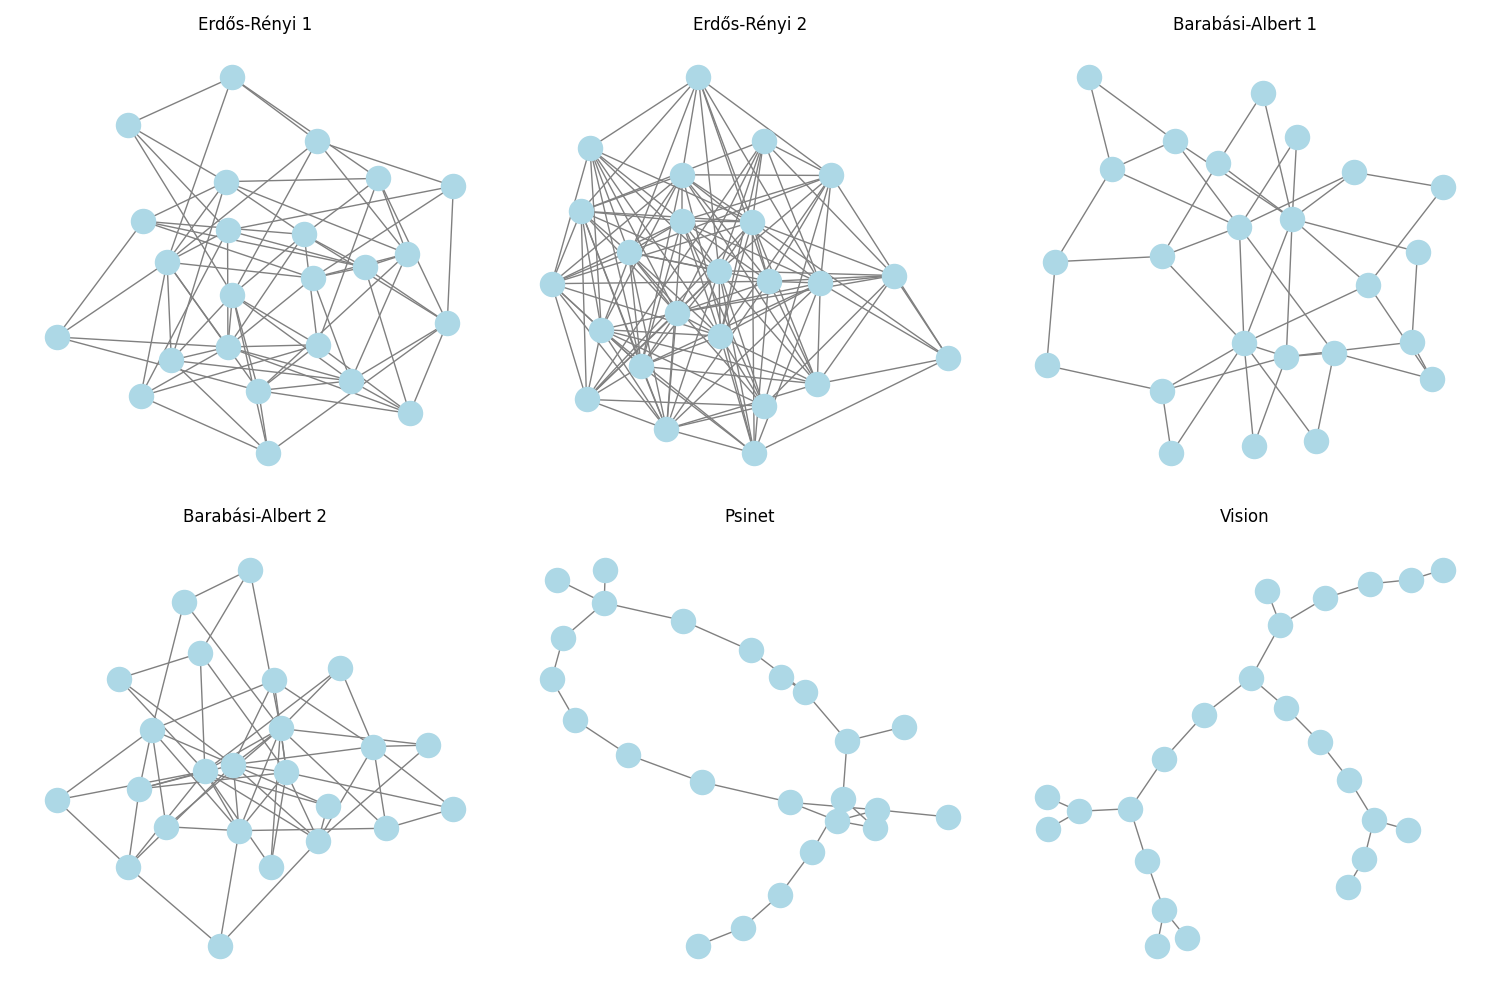
\includegraphics[width=0.8\linewidth]{images/Topology set/24.png}
    \caption{Proposed topologies (24 nodes)}
    \label{fig:24_prop}
\end{figure}

\begin{figure}
    \centering
    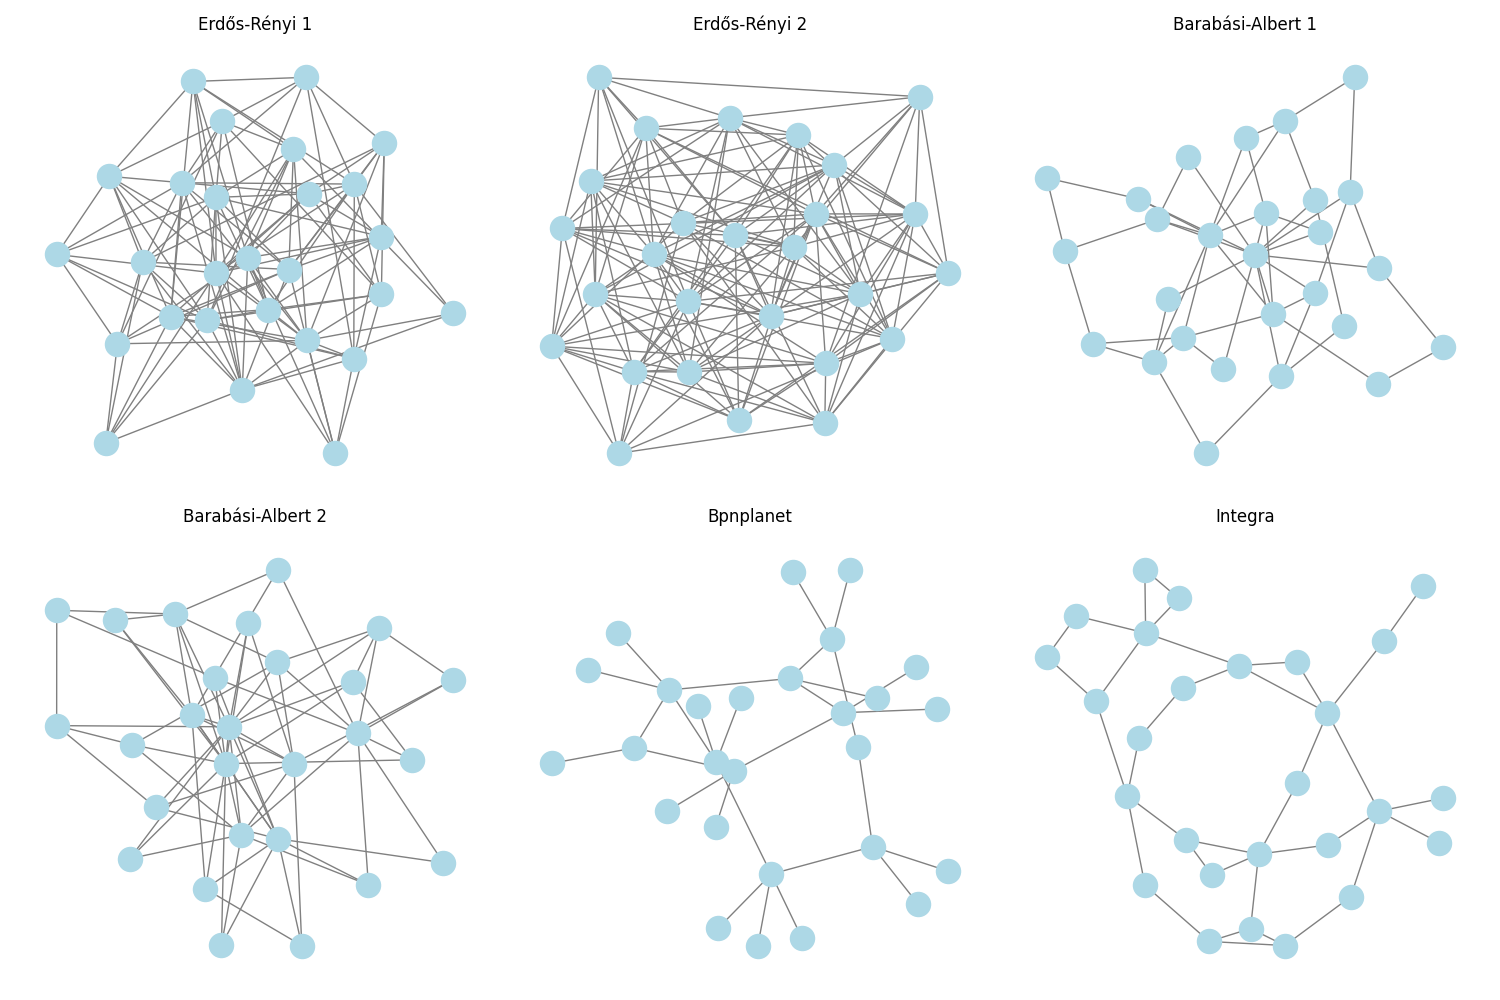
\includegraphics[width=0.8\linewidth]{images/Topology set/27.png}
    \caption{Proposed topologies (27 nodes)}
    \label{fig:27_prop}
\end{figure}

\newpage